% Chapter 3
\chapter{Library Implementation}
\label{chap:Chapter3}

This chapter will be dedicated to describing in detail how the library was developed. The theory and calculus involved in structuring a \gls{CVNN} will be described as some, fundamental notions like forwarding a signal and training a \gls{CVNN}. Afterwards, it will be briefly addressed how the library is structured followed by the main algorithms implemented to perform the necessary calculus related to \gls{CVNN} tasks. This chapter will be wrapped up with some guidelines on how to operate with the library.

\section{Theory \& Calculus}
The development of this library required some fundamental notions of complex analysis, therefore while going through the theory behind the dynamics of a \gls{CVNN}  in this library, essential Complex Analysis concepts will also be presented. First, establishing some fundamental concepts regarding \gls{ANN}, second, how a \gls{CVNN} forwards a signal, including a small discussion around complex activation functions, and third, how a \gls{CVNN} learns with the fully complex back-propagation algorithm.

A majority of the fundamental notions involved in this chapter come from Wintinger Calculus \parencite{wirtinger1927formalen}.

\subsection{Fundamentals}
\label{subsec:fundamentals}
A \gls{ANN} can have a high-level representation  as a multivariate function whose parameters are its weights and biases.

\begin{equation}
	\mathbf{y} = f_{w_{1}, w_{2}, ..., b_{1}, b_{2}, ...}(\mathbf{x}),
	\label{eq:network}
\end{equation}
where $ f $ is the function that represents the network, $ w_{i} $, $ b_{i} $ its weights and biases respectively, $ \mathbf{x} $ the input features of a certain data point to be forwarded through the network, yielding the output features $ \mathbf{y} $. 

\gls{ANN} are composed of layers which take a set of $ n_i $ input features, perform some operation on these features and output a set of $ n_o $ output features. Such operations, in the real domain, consist of e.g. computing a weighted sum or convolution. One can also visualize a layer as a function,

\begin{equation}
	\mathbf{y}^{(l)} = g_{w_{1}, w_{2}, ..., b_{1}, b_{2}, ...}(\mathbf{x}^{(l)}),
	\label{eq:layer}
\end{equation}
being $ g $ the function that represents the layer, $ \mathbf{y}^{(l)} $ the input and $ \mathbf{x}^{(l)} $ the output features of a layer $ l $, and $ w_{i} $, $ b_{i} $ the weights and biases, respectively, of the layer (not necessarily the same set as in equation (\ref{eq:network})). 

Now, functions $ f $ and $ g $ are the same only if the \gls{ANN} is composed of one layer. \gls{ANN} typically contain multiple layers where mathematically speaking,

\begin{equation}
	\mathbf{y} = g^{(L)} \circ ... \circ g^{(2)} \circ g^{(1)}(\mathbf{x}),
	\label{eq:layer_comp_network}
\end{equation}
with $ \circ $ denoting the chain composition operator, $ L $ being the total number of layers in the \gls{ANN}, and $ f(\mathbf{x}) = g^{(L)} \circ ... \circ g^{(2)} \circ g^{(1)}(\mathbf{x}) $. Figure~\ref{fig:raw_net} depicts a high-level representation of an \gls{ANN} according to the formalism used.

\begin{figure}[htbp]
	\centering
	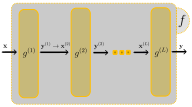
\includegraphics[width=0.9\textwidth]{ch3/assets/raw_net.png}
	\caption{High-level representation of an ANN through function composition showing the dynamics of input $ \x $ all the way to the output $ y $ through $ L $ layers. }
	\label{fig:raw_net}
\end{figure}

\subsubsection{Processing Unit}
Layers contain an array of neurons or processing units (for short, unit). Each unit is capable of accessing the entire length of input features to that layer and it is the element that possesses the parameters of the network (weights and biases). The layer's number of output features is mediated by the number of units present in that layer.

Since each layer has its own sets of units, to keep track of all parameters, we will establish the following definitions:

\begin{itemize}
	\item $ \w{l}{i} $ - weights of neuron $ i $ of layer $ l $. Weights can be a scalar, vector, matrix or generally speaking, a tensor;
	\item $ \bi{l}{i} $ - scalar bias value of neuron $ i $ of layer $ l $;
	\item $ \ints{l} $ - number of input features of layer $ l $;
	\item $ \outs{l} $ - number of units or number of output features of layer $ l $;
	\item $ \intsp{l} $ - input feature shape of layer $ l $;
	\item $ \outsp{l} $ - output feature shape of layer $ l $.
\end{itemize}

Upon receiving the input features, unit $ i $ in layer $ l $ will perform some computation expressed by a function $ \paf{l} $, resulting in one output feature per unit. The quintessential example of such computation is the weighted sum, where if a neuron receives a vector of layer input features $ \x' $,

\begin{equation}
	\pact{l}{i} = \paf{l}(\w{l}{i}, \bi{l}{i}, \x^{(l)}) = \w{l}{i} \cdot \x^{(l)} + \bi{l}{i},
	\label{eq:pact_weighted_sum}
\end{equation}
being $ \paf{l}:  \mathbb{R}^{\ints{l}} \rightarrow \mathbb{R} $, $ \pact{l}{i} $ the pre-activation value of neuron $ i $ of layer $ l $ and "$ \cdot $" denotes the dot product. In this example, $ \pact{l}{i} $ happens to be a scalar\footnote{In general terms, these quantity can also be a tensor depending on the pre-activation operation.} and it was decided to name it pre-activation since the last step of the processing unit computation, is the application of an activation function.

The derivative of the activation function $ \af{l} $ must yield a limited function. This function will receive the pre-activation value from a unit $ i $ of layer $ l $ to filter them to an appropriate range for the network, returning the final output feature or the activation value $ \act{l}{i} $ of the unit,

\begin{equation}
	\act{l}{i} = \af{l}(\pact{l}{i}),
	\label{eq:act}
\end{equation}
where $ \act{l}{i} $ has the same dimensions as $ \pact{l}{i} $. Two standard examples of $ \af{l} $ where $ \af{l}: \mathbb{R} \rightarrow \mathbb{R} $ can be, for instance, the sigmoid function $ \sigma $ or hyperbolic tangent $ \tanh $ operating. The layer $ l $'s output will be a vector of length $ \outs{l} $ containing all $ \act{l}{i} \ \text{for} \ i = 1, 2, ..., \outs{l} $. On a side note, one can see that this process inside a unit is also a composition of functions,

\begin{equation}
	\act{l}{i} = \af{l} \circ \paf{l}(\w{l}{i}, \bi{l}{i}, \x^{(l)})
	\label{eq:comp_act}
\end{equation}

The main gist of a \gls{RVNN} when compared to a \gls{CVNN} is that $ \w{l}{i} \in \mathbb{C}^{\intsp{l}} $ and $ \bi{l}{i} \in \mathbb{C} $ for $ i = 1, 2, ..., \outs{l} $. This small modification on the network's parameters carries out major consequences in the traditional dynamics of \gls{RVNN}.

\subsection{Signal Forwarding}
To forward a signal through an \gls{ANN}, one must define the layers of the network, i.e. defining the functions $ g^{l} $ for $ l = 1, 2, ..., L $ where $ L $ is the number of layers in the network, and calculate the chain composition of functions given input $ \x $ as expressed in equation (\ref{eq:layer_comp_network}). To define the function $ \actf{l} $ where $ \actf{l}: \mathbb{R}^{\intsp{l}} \rightarrow \mathbb{R}^{\outsp{l}} $, one must first understand its action. Since a layer $ l $ will return $ \outs{l} $ output features then,

\begin{multline}
	\y^{(l)} = \actf{l}(\x^{(l)}) = \\ 
	[\af{l} \circ \paf{l}(\w{l}{1}, \bi{l}{1}, \x^{(l)}),
		\af{l} \circ \paf{l}(\w{l}{2}, \bi{l}{2}, \x^{(l)}),
		...,
		\af{l} \circ \ \paf{l} (\w{l}{N}, \bi{l}{N}, \x^{(l)}) ]
\end{multline}
with $ N = \outs{l} $. Indexing the output features yields,

\begin{equation}
	\y^{(l)} = \act{l}{i} = \af{l} \circ \paf{l}(\w{l}{i}, \bi{l}{i}, \x^{(l)}).
\end{equation}
With this in mind, one no longer needs the abstract function $ \actf{l} $. The layer $ l $ can be defined by the pre-activation function $ \paf{l} $ and the activation function $ \af{l} $. It is important to emphasize that, due to abuse of notation, it is not clear that $ \paf{l} $ and $ \af{l} $ can be different functions from $ \paf{l+1} $ and $ \af{l+1} $, which in fact can in cases where the network has multiple layers. If $ L = 1 $ forwarding a signal through the network can be trivial like so,

\begin{equation}
	\y_i =  \act{1}{i} = \af{1} \circ \paf{1} (\w{1}{i}, \bi{1}{i}, \x).
\end{equation}
For a generic $ L $, the entire forward dynamic is summarized as,

\begin{equation}
	\act{l}{i} = \af{l} \circ \paf{l} (\w{l}{i}, \bi{l}{i}, \act{l-1}{j})
\end{equation}
where $ \act{l=0}{i} = \x_i $ being the input to the \gls{ANN} ($ l = 0 $ is a virtual layer) and $ \act{l=L}{i} = \y_i $ the prediction of the network. The generic indices $ i, j $, are used to represent that different layers can have different lengths of input and output features, i.e., typically $ \ints{l} \neq \ints{l-1} $. Additionally, the number of input features of each layer must be equal to the number of output features of the previous layer, i.e. $ \ints{l} = \outs{l-1} $. Figure~\ref{fig:complete_net}, presents an illustrative summary of the notation and dynamics addressed up until this point.

\begin{figure}[htbp]
	\centering
	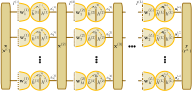
\includegraphics[width=1.0\textwidth]{ch3/assets/complete_net.png}
	\caption{Base architecture of a neural and framing with the formalism introduced in this chapter. In this illustration, $  N = \outs{1} $, $ M = \outs{2}$ and $ K = \outs{L} $. To not make the illustration to dense , the bias parameter was omitted, nevertheless, its framing is analogous to the weights.}
	\label{fig:complete_net}
\end{figure}

\subsection{Complex Activation Functions}
At a high-level, this procedure applies for both \gls{RVNN} and \gls{CVNN}. The major difference happens when one looks at the function $ \paf{l} $ and $ \af{l} $ since now they map values in the complex domain. Proceeding to examining the example of the pre-activation function of the weighted sum in equation (\ref{eq:pact_weighted_sum}) in the complex domain $ \mathbb{C} $. The first instance where this domain offers some non-linearity in the calculations, is in the product between two complex numbers inside the scalar product between $ \w{l}{i} $ and $ \x' = \act{l-1}{j} $.  Considering two complex numbers $ z_1 = x_1 + iy_1 $ and $ z_2 = x_2 + iy_2 $, their multiplication can be expressed in function of each one's real and imaginary components,

\begin{equation}
	z = z_1 z_2 = ( x_1 x_2 - y_1 y_2 ) + i( x_1 y_2 + y_1 x_2 ),
\end{equation}
where $ \Imag{z_1} $ and $\Imag{z_2} $ have an important role in modulating $ \Real{z} $. The second instance is in choosing an activation function for the network.

From this point onward, it is important to start considering the properties of complex numbers and its consequences on a \gls{CVNN}. Since the weights and biases are now complex, even if  the values of the input features carry no imaginary component, the forwarded signal will eventually pick up an imaginary component.

For a function to be viable candidate as an \gls{CAF} $ \af{l}: \mathbb{C}^{\outsp{l}} \rightarrow \mathbb{C}^{\outsp{l}} $ for a given layer $ l $, its derivative needs to have a limited codomain. In the real domain, the previously given examples of $ \sigma $ and $ \tanh $ are actually both limited in its original form and its derivative. However, if we take for instance function $ \sigma $ and provide it a complex argument, it will result in a function that does not have a limited codomain, nor a limited derivative, due to the exponentiation of complex numbers. A typical work around is to define a Real-Imaginary-Type function or Split-Function, as shown in equation (\ref{eq:split_func}).

\begin{equation}
	\af{l}(z) = \af{l}_{r}(\Real{z}) + i \af{l}_{r}(\Imag{z}),
	\label{eq:split_func}
\end{equation}
with $ \af{l}_{r}:  \mathbb{R}^{\outsp{l}} \rightarrow \mathbb{R}^{\outsp{l}} $ a function with limited derivative. Given that $ \af{l}_{r} $ is limited, ensures that  $ \af{l} $ and its derivative is also limited, therefore, a viable candidate as a \gls{CAF}.

A group of split functions can be created based on real-valued \gls{AF} which are present in the library but also two more viable \gls{CAF}. The library also implements the zReLU function

\begin{equation}
	\af{l}(z) = 
	\begin{cases}
		z \ \text{if} \  0 \leqslant \arg(z) \leqslant \frac{\pi}{2} \\
		0 \  \text{otherwise}
	\end{cases},
\end{equation}
Additionally, it also implements an adaptation of the cardioid curve, as a function,

\begin{equation}
	\af{l}(z) = \dfrac{1}{2} ( 1 + \cos(\arg(z)) ) z
\end{equation}
Both functions being explicitly dependent on the phase of $ z $ and with only its derivative as a limited function.

\subsection{Complex Back-Propagation}
In section \ref{subsec:fundamentals} it was defined a set of functions and composition of functions that, at the time, seemed to be just some abstraction. However, these functions will be important for implementing an algorithm based on the gradient descent optimization method \parencite{cauchy1847}, that will make it possible for the \gls{CVNN} to learn through data. This requires knowledge in Complex Analysis, specifically complex function derivatives, and using the complex chain rule in the composition of functions to implement Complex Back-Propagation \parencite{rumelhart1986}.

Before going through complex differentiation, let us quickly define a complex loss function. Although a simple concept, it is crucial for implementing complex gradient descent (or optimization algorithms in general).

Typically, in the real domain, one can define the \gls{RVNN} loss function as,

\begin{equation}
	\loss_n = \left( \act{L}{n} - r_n \right)^2,
	\label{eq:error_cp}
\end{equation}
where $ \loss_n $ represents the error of neuron $ n $ given last layer's activation $ \act{L}{n} $ and $ r_n $ the target output feature result (from the dataset). A mean or a sum can be performed along the flatten values of $ \loss_n $ for instance to a single value of the loss function expressed in equation (\ref{eq:losstotal}) 

\begin{equation}
	\loss = \sum_{n}^{\outs{L}} \loss_n,
	\label{eq:losstotal}
\end{equation}

In the complex domain, not a lot changes in the error expression $ \loss_n: \mathbb{C}^{\outsp{L}} \rightarrow \mathbb{R}^{\outsp{L}} $, since a complex codomain is not going to be considered. The complex error function can be,

\begin{equation}
	\loss_n = \left| \act{L}{n} - r_n \right|^2,
	\label{eq:cerror}
\end{equation}
with $ \left| \act{L}{n} - r_n \right| $ being the absolute value of the complex number resultant from $ \act{L}{n} - r_n $.

\subsubsection{Complex differentiation}
Differentiating a complex function is going to be the most important task to perform in the complex gradient descent (as a consequence, complex back-propagation), and it is important to recognize certain types of complex functions.

In complex analysis, an Holomorphic function is a function that obeys the Cauchy-Riemann equations \parencite{Cauchy1814}. Given a function $ f(z) = u(x,y) + iv(x,y) $ where $ z = x + iy $, the Cauchy-Riemann equations read,

\begin{equation}
	\der{u}{x} = \der{v}{y}, \ \der{u}{y} = -\der{v}{x}.
	\label{eq:cr}
\end{equation}
If such a function $ f $ obeys these equations, then its derivative with respect to $ z $ can be easily taken according to,

\begin{equation}
	\der{f}{z} = \der{u}{x} + i\der{v}{x}.
	\label{eq:cr_der}
\end{equation}
However, in this scenario of \gls{CVNN}, functions typically do not obey equations in (\ref{eq:cr}). These functions are called non-holomorphic, and equation in (\ref{eq:cr_der}) no longer holds true. To compute the derivative of a non-holomorphic function, one must first layout the chain rule between a complex function and its argument's real and imaginary part like so,

\begin{equation}
	\begin{cases}
		\der{f}{z} = \der{f}{x}\der{x}{z} + \der{f}{y}\der{y}{z} \\
		\\
		\der{f}{\conj{z}} = \der{f}{x}\der{x}{\conj{z}} + \der{f}{y}\der{y}{\conj{z}}
	\end{cases},
	\label{eq:complex_chain_der}
\end{equation}
being $ \conj{z} $ the complex conjugate of $ z $. Here, we are considering also the derivative with respect to $ \conj{z} $ because both $ x $ and $ y $, have an implicit dependence in $ z $ and $ \conj{z} $ as show in equation (\ref{eq:xydepz}),

\begin{equation}
	\begin{cases}
		x = \dfrac{z + \conj{z}}{2} \\
		\\
		y = \dfrac{z - \conj{z}}{2i}
	\end{cases}.
	\label{eq:xydepz}
\end{equation}
We can use this dependency to simplify equation in (\ref{eq:complex_chain_der}) yielding,
\begin{equation}
	\begin{cases}
		\der{f}{z} = \dfrac{1}{2} \left( \der{f}{x} - i\der{f}{y} \right) \\
		\\
		\der{f}{\conj{z}} = \dfrac{1}{2} \left( \der{f}{x} + i\der{f}{y} \right)
	\end{cases}.
	\label{eq:complex_chain_der_simp}
\end{equation}
These derivative expressions are valid for both holomorphic and non-holomorphic functions, however, one would see that the second is null for the holomorphic case. This is an important fact since, computationally-wise, if one knows from the start that a function is holomorphic: calculating its conjugate derivative is not necessary; a more straight-forward expression can be taken; last but not least, no need for storing unnecessary null data regarding the conjugate derivative and perform further calculations with just zeros.

The function definitions established in Section \ref{subsec:fundamentals}, will help categorize each one to simplify the back-propagation algorithm as much as possible.

\subsubsection{Holomorphic \& Non-Holomorphic functions in a \gls{CVNN}}
\label{subsubsec:holo_non_holo}
\paragraph{Pre-Activation Function $ \paf{l} $} 
The most common example of a $ \paf{l} $, is the (complex) weighted sum showed in equation (\ref{eq:pact_weighted_sum}), which for the sake of this library, only layer logics based on the weighted sum will be used (common weighted sum and convolution). First point is to know if such function is holomorphic, therefore, one needs to apply the Cauchy Riemann equations in \ref{eq:cr}. If it proves that the complex summation function $ f_1(z) = z + z_0 $ and the complex multiplication function $ f_2(z) = z z_0 $ are holomorphic, due to the properties of holomorphic functions \parencite{wirtinger1927formalen}, we can prove that the sum of complex products, is holomorphic (which is what a weighted sum is). For $ f_1 $ there is,

\begin{equation}
	\begin{cases}
		u(x,y) = x + x_0 \Rightarrow \der{u}{x} = 1, \ \der{u}{y} = 0 \\
		\\
		v(x,y) = y + y_0 \Rightarrow \der{v}{x} = 0, \ \der{v}{y} = 1
	\end{cases},
	\label{eq:cauchypactholo}
\end{equation}
with $ z_0 = x_0 + iy_0 $. Equation (\ref{eq:cauchypactholo}) shows that the summation function is holomorphic. For $ f_2 $,

\begin{equation}
	\begin{cases}
		u(x,y) = x  x_0 - y y_0 \Rightarrow \der{u}{x} = x_0, \ \der{u}{y} = -y_0 \\
		\\
		v(x,y) = x y_0 + y x_0 \Rightarrow \der{v}{x} = y_0, \ \der{v}{y} = x_0
	\end{cases},
\end{equation}
where Cauchy-Riemann Equations also hold. Therefore yields,

\begin{equation}
	\paf{l}(\w{l}{i}, \bi{l}{i}, \act{l-1}{j}) = \w{l}{i} \cdot \act{l-1}{j} + \bi{l}{i}, \  \forall\w{l}{i}, \act{l-1}{j}, \bi{l}{i} \in \mathbb{C},
\end{equation}
being an holomorphic function. According to equation (\ref{eq:cr_der}), one can determine what are going to be the relevant partial derivatives for the back-propagation algorithm in equation (\ref{eq:reldel}),

\begin{equation}
	\begin{cases}
		\der{\paf{l}}{\act{l-1}{j}} = \w{l}{i} \\
		\\
		\der{\paf{l}}{\w{l}{i}} = \act{l-1}{j} \\
		\\
		\der{\paf{l}}{\bi{l}{i}} = 1 \\
		\\
		\left( \der{\paf{l}}{\cact{l-1}{j}} = \der{\paf{l}}{\cw{l}{i}} = \der{\paf{l}}{\cbi{l}{i}} = 0 \right)
	\end{cases}.
	\label{eq:reldel}
\end{equation}

\paragraph{Complex Activation Functions $ \af{l} $}
Considering the set of activation functions present in this library, all happen to be non-holomorphic with the exeption of zReLU. By reviewing the split-function in equation (\ref{eq:split_func}), one proves that all split-functions are non-holomorphic, by applying the Cauchy-Riemann Equation in equation (\ref{eq:creq_split}),

\begin{equation}
	\begin{cases}
		u(x,y) = u(x) = \af{l}_r(\Real{z}) \Rightarrow \der{u}{x} = \der{\af{l}_r}{x}, \ \der{u}{y} = 0 \\
		\\
		v(x,y) = v(y) = \af{l}_r(\Imag{z}) \Rightarrow \der{v}{x} = 0, \ \der{v}{y} = \der{\af{l}_r}{y}
	\end{cases}.
	\label{eq:creq_split}
\end{equation}
Given the explicit dependency of $ u = u(x) $ and $ v = v(y) $, its derivatives with respect to $ x $ and $ y $ respectively, are always going to be different aside from when $ x = y $. Nevertheless, since the entire domain of the split-functions is used, differentiation is performed with equation
(\ref{eq:complex_chain_der_simp}) resulting in,

\begin{equation}
	\begin{cases}
		\der{\af{l}}{z} = \dfrac{1}{2} \left( \der{\af{l}_r}{x} + \der{\af{l}_r}{y} \right) \\
		\\
		\der{\af{l}}{\conj{z}} = \dfrac{1}{2} \left( \der{\af{l}_r}{x} - \der{\af{l}_r}{y} \right)
	\end{cases}.
\end{equation}

\paragraph{Complex Loss Function $ \af{l} $}
Differentiating the complex error function in equation (\ref{eq:cerror}) is the starting point to determine the entire gradients of the network, since it is going to dictate what is the downward direction to optimize the error for each neuron, and as a consequence, downward direction in the entire loss function surface.

First checking if the error function in equation (\ref{eq:cerror}), is holomorphic, and for simplicity, considering $ \norm{\act{L}{n} - r_n}^2 = \norm{z}^2 = x^2 + y^2 $,

\begin{equation}
	\begin{cases}
		u(x,y) =  = x^2 + y^2 \Rightarrow \der{u}{x} = 2x, \ \der{u}{y} = 2y \\
		\\
		v(x,y) = 0 \Rightarrow \der{v}{x} = 0, \ \der{v}{y} = 0
	\end{cases}.
\end{equation}
So this tells that the complex absolute value function is a non-holomorphic function, therefore, the loss function is only holomorphic for error values of zero (which is going to be never a reachable value). One needs to consider the non-holomorphic derivatives, which after some basic algebra yields,

\begin{equation}
	\begin{cases}
		\der{\loss_n}{\act{L}{n}} = \cact{L}{n} - \conj{r}_n \\
		\\
		\der{\loss_n}{\cact{L}{n}} = \act{L}{n} - r_n
	\end{cases}.
\end{equation}

\subsubsection{Complex Chain Rule}
To implement an optimization method based on the complex gradient descent, only rests to define a chain rule for propagating derivatives. 

Supposing two generic complex functions $ A $ and $ B $ have a dependency in $ z $ and in $ \conj{z} $ in case $ A $ and $ B $ are non.holomorphic. If there is a complex function $ C = B \circ A $, then to compute the chain rule, one must consider $ z $ and $ \conj{z} $. So, the chain rule for $ B \circ A $ where both functions are non-holomorphic is,

\begin{equation}
	\begin{cases}
		\der{(B \circ A)}{z} = \der{B}{A}\der{A}{z} + \der{B}{\conj{A}}\der{\conj{A}}{z} \\
		\\
		\der{(B \circ A)}{\conj{z}} = \der{B}{A}\der{A}{\conj{z}} + \der{B}{\conj{A}}\der{\conj{A}}{\conj{z}} \\
	\end{cases}
	\label{eq:AB_nonholo}
\end{equation}
where properties such as,

\begin{equation}
	\begin{cases}
		\der{\conj{A}}{z} = \text{conj}\group{\der{A}{\conj{z}}} \\
		\\
		\der{\conj{A}}{\conj{z}} = \text{conj}\group{\der{A}{z}}
	\end{cases},
	\label{eq:comp_conj_div}
\end{equation}
hold for these derivatives where, for readability, $ \text{conj}(z) = \conj{z} $. However, if $ A $ is holomorphic,

\begin{equation}
	\begin{cases}
		\der{(B \circ A)}{z} = \der{B}{A}\der{A}{z} \\
		\\
		\der{(B \circ A)}{\conj{z}} = \der{B}{\conj{A}}\der{\conj{A}}{\conj{z}} \\
	\end{cases},
\end{equation}
else if $ B $ is holomorphic,
\begin{equation}
	\begin{cases}
		\der{(B \circ A)}{z} = \der{B}{A}\der{A}{z} \\
		\\
		\der{(B \circ A)}{\conj{z}} = \der{B}{A}\der{A}{\conj{z}} \\
	\end{cases},
	\label{eq:B_holo}
\end{equation}
else if $ A $ and $ B $ are both holomorphic,

\begin{equation}
	\begin{cases}
		\der{(B \circ A)}{z} = \der{B}{A}\der{A}{z} \\
		\\
		\der{(B \circ A)}{\conj{z}} = 0 \\
	\end{cases}.
\end{equation}
These expressions are very much important in the Complex Back-Propagation algorithm as it will become apparent.

\subsubsection{Complex Gradient Descent \& Back-Propagation}
In the task of optimizing a neural network based on the gradient descent optimization method, the objective is to determine the gradient of the loss function like so,

\begin{equation}
	\begin{cases}
		\der{\loss}{\w{l}{i}}  = \der{\group{\loss \circ f}}{\w{l}{i}} = 
		\der{\group{\loss \circ \group{g^{(L)} \circ ... \circ g^{(2)} \circ g^{(1)}}}}{\w{l}{i}} \\
		\\
		\der{\loss}{\bi{l}{i}}  = \der{\group{\loss \circ f}}{\bi{l}{i}} = 
		\der{\group{\loss \circ \group{g^{(L)} \circ ... \circ g^{(2)} \circ g^{(1)}}}}{\bi{l}{i}} \\
	\end{cases},
\end{equation}
since $ g^{l} = \af{l} \circ \paf{l} $ and the only adjustable parameters of the network are $ \w{l}{i} $ and $ \bi{l}{i} $ for every $ l = 1, 2, ..., L $ and $ i = 1, 2, ..., \ints{l} $\footnote{The index $ i $ is implicitly dependent on $ l $}.

This derivative is not straightforward to determine, because the only starting point is from the loss function it to optimize it with an explicit dependence on only last layer's activation $ \act{L}{n} $. The way one determines the full derivative is by applying the back-propagation algorithm.

First, the loss function's dependency with respect to last layer's weights and biases, $ \w{L}{n} $ and $ \bi{L}{n} $ respectively is,

\begin{equation}
	\begin{cases}
		\der{\loss}{\w{L}{n}} = \der{\group{\loss \circ \act{L}{n}}}{\w{L}{n}} \\
		\\
		 \der{\loss}{\bi{L}{n}} = \der{\group{\loss \circ \act{L}{n}}}{\bi{L}{n}}
	\end{cases}.
\end{equation}
Because of the properties mentioned in equation (\ref{eq:comp_conj_div}) and the fact that $ \func[\loss]{\set{C}^{\outsp{L} \otimes \outs{L}}}{\set{R}} $ results in,

\begin{equation}
	\begin{cases}
		\der{\loss}{\cw{l}{i}} = \text{conj}\group{\der{\loss}{\w{l}{i}}} \\
		\\
		\der{\loss}{\cbi{l}{i}} = \text{conj}\group{\der{\loss}{\bi{l}{i}}}
	\end{cases}.
\end{equation}

Going back to section~\ref{subsubsec:holo_non_holo}, $ \act{L}{n} $  as function of $ \pact{L}{n} $, is a non-holomorphic function just like $ \loss(\act{L}{n})  $. Therefore, one can use equation in (\ref{eq:AB_nonholo}) to determine the derivative compositions,

\begin{equation}
	\begin{cases}
		\der{\loss}{\w{L}{n}} = \der{\loss}{\act{L}{n}}\der{\group{\act{L}{n} \circ \pact{L}{n}}}{\w{L}{n}} + \der{\loss}{\cact{L}{n}}\der{\group{\cact{L}{n} \circ \pact{L}{n}}}{\w{L}{n}} \\
		\\
		\der{\loss}{\bi{L}{n}} = \der{\loss}{\act{L}{n}}\der{\group{\act{L}{n} \circ \pact{L}{n}}}{\bi{L}{n}} + 	\der{\loss}{\cact{L}{n}}\der{\group{\cact{L}{n} \circ \pact{L}{n}}}{\bi{L}{n}} 
	\end{cases}.
\end{equation}
Nevertheless, $ \act{L}{n}(\pact{L}{n}) $ (result of function $ \paf{L} $) does not have an explicit dependency in $ \w{L}{n} $ but $ \pact{L}{n}(\w{L}{n}, \bi{L}{n}, \act{L-1}{m}) $ has (result of function $ \af{L} $). As  shown in section~\ref{subsubsec:holo_non_holo} that $ \pact{L}{n} $ is holomorphic so it is possible to apply equation in (\ref{eq:B_holo}). Establishing the following definitions in equation (\ref{eq:lossdef}) beforehand to make the equations more readable,

\begin{equation}
	\begin{cases}
		\ploss{L}{n} \equiv \der{\loss}{\act{L}{n}}\der{\act{L}{n}}{\pact{L}{n}} \\
		\\
		\pcloss{L}{n} \equiv \der{\loss}{\cact{L}{n}}\der{\cact{L}{n}}{\pact{L}{n}} \\
	\end{cases}.
	\label{eq:lossdef}
\end{equation}
The derivative of the loss function with respect to the weights and biases of the last layer is,

\begin{equation}
	\begin{cases}
		\der{\loss}{\w{L}{n}} = \group{\ploss{L}{n}+ \pcloss{L}{n}}\der{\pact{L}{n}}{\w{L}{n}} \\
		\\
		\der{\loss}{\bi{L}{n}} = \group{\ploss{L}{n} + \pcloss{L}{n}}\der{\pact{L}{n}}{\bi{L}{n}} \\
	\end{cases}.
\end{equation}

Now the next step is to determine the derivative of the loss function with respect to the weights and biases of the previous to last layer represented in equation (\ref{eq:prev_layer_wb}),

\begin{equation}
	\begin{cases}
		\der{\loss}{\w{L-1}{m}} = \group{\ploss{L-1}{m} + \pcloss{L-1}{m}}\der{\pact{L-1}{m}}{\w{L-1}{m}} \\
		\\
		\der{\loss}{\bi{L-1}{m}} = \group{\ploss{L-1}{m} + \pcloss{L-1}{m}}\der{\pact{L-1}{m}}{\bi{L-1}{m}} \\
	\end{cases},
	\label{eq:prev_layer_wb}
\end{equation}
where in this expression,  all values are known aside from $ \ploss{L-1}{m} $ and $ \pcloss{L-1}{m} $.

The key to the back-propagation algorithm, is determining the derivative of the loss function with respect to the previous to last layer's activation such that one can keep iterating backwards until the input layer ($ l = 1 $) is reached. Therefore yields,

\begin{equation}
	\der{\loss}{\act{L-1}{m}} = \sum_{n} \left[ \group{\ploss{L}{n} + \pcloss{L}{n}}\der{\pact{L}{n}}{\act{L-1}{m}} \right],
	\
	\der{\loss}{\cact{L-1}{m}} =  \text{conj}\group{\der{\loss}{\act{L-1}{m}}} \\
	\label{eq:back_prop}
\end{equation}
where the sum over the units $ n $, means that each neuron $ m $ of layer $ L-1 $ contributes equally to every neuron's activation of layer $ L $.

Now one can use equation in (\ref{eq:back_prop}) to determine the values of $ \ploss{L-1}{m} $ and $ \pcloss{L-1}{m} $ and insert them in equation (\ref{eq:prev_layer_wb}) to propagate the derivatives backwards.

This Complex Back-Propagation is implemented by the proposed library and a summary can be visualized in Figure~\ref{fig:backprop}. In upcoming sections, some small technical details regarding the implementation of this algorithm will be discussed and some other operations relevant to \gls{CVNN} modeling.

\begin{figure}[htbp]
	\centering
	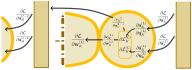
\includegraphics[width=1.0\textwidth]{ch3/assets/cp_backprop.png}
	\caption{Depiction summarizing the complex back-propagation algorithm, at the neuron level, used in Renplex. Arrows indicate calculations and one can see that, computational-wise, the majority of the derivatives can be calculated in parallel. Derivatives related to the bias were omitted for a more concise illustration and here $ M = \outs{L-1} $ and $ K = \outs{L} $}.
	\label{fig:backprop}
\end{figure}

\section{Structure of the Library}

The library is structured in 8 modules:

\begin{itemize}
	\item \texttt{act} : Activation function definitions and interface for computing activation values;
	\item \texttt{cvnn}: Core module that contains structures and tools for modulating \gls{CVNN} architectures.
	\item \texttt{dataset}: Interface for processing datasets automatically;
	\item \texttt{err}: Minimal error handling enumerations;
	\item \texttt{init}: Enumerations for computing layer initialization techniques;
	\item \texttt{input}: Enumerations for handling static input and output features shapes for layers;
	\item \texttt{math}: Various mathematical utilities concerning, for instance, complex float, matrix definition and operations and random number generation;
	\item \texttt{opt}: Definition and computing loss function and its derivatives.
\end{itemize}

A brief overview on the core module \texttt{cvnn}.

\paragraph{\texttt{cvnn} Module}
The core module \texttt{cvnn}, only possesses two additional modules: \texttt{layer} and \texttt{network}. \texttt{layer} module is arguably the most important as it contains all the layers implemented in the library each one with its own logic, being:

\begin{itemize}
	\item \texttt{DenseCLayer}: Contains a matrix of weights, vector of biases (as many as there is units), and an activation function. It represents a fully connected layer that performs the common weighted sum in equation (\ref{eq:pact_weighted_sum}) given a vector of scalar input features;
	\item \texttt{Flatten}: Flattens out a vector of matrix input features into a vector of scalar input features;
	\item \texttt{ConvCLayer}: Contains a matrix of weights (filters/kernels), a vector of biases and an activation function. This layer computes the convolution between every matrix input feature against every filter. The number of filters will dictate the number of output features (matrices);
	\item \texttt{Reduce}: A generalized pooling operation that asks for the user the operation to be applied on each block of each input feature matrix. Each matrix block of every input feature will be reduced into a scalar for down-sampling data.
\end{itemize}

The \texttt{network} module only defines the \texttt{struct} of a network, being a vector of layers, and underlying operations such as running the complex gradient descent optimization for a batch of data, adjusting the weights of the layers accordingly, calculating loss and accuracy, and forwarding and intercepting signals.

Having this quick layout of the library, the main implemented features, operations and critical algorithms will be addressed.

More details on the structure of the library can be viewed in the Github repository \href{https://github.com/Pxdr0-A/renplex.git}{Pxdr0-A/renplex.git}, it is also published in the crates.io, the official package manager for Rust in \href{https://crates.io/crates/renplex}{https://crates.io/crates/renplex}. Documentation for this library can also be accessed in \href{https://docs.rs/renplex/0.1.1/renplex/}{https://docs.rs/renplex/0.1.1/renplex/}.

\section{Main Implementations}
To give some insights on the operation and performance of the library, in this section, there will be an overview on the most critical tasks executed in the library.

\subsection{Matrix-Vector Multiplication}

The Rust implementation for this operations goes as follows:

\begin{lstlisting}[caption=Onverview on the Matrix-Vector multiplication implemented in the Renplex Library using Rust.]
	pub fn mul_slice(
		&self, 
		rhs: &[T]
	) -> Result<Vec<T>, OperationError> {
		
		// error handling
		...
		
		// map rows of the matrix
		let res = self.rows_as_iter().map(|elm| {
			// create a row and vec iterator
			elm.into_iter()
			.zip(rhs.iter())
			// perform scalar product
			.fold(T::default(), |acc, elm| { 
				acc + (*elm.0 * *elm.1) 
			})
		}).collect::<Vec<_>>();
		
		Ok(res)
	}
\end{lstlisting}

Here, the slice \texttt{rhs:\&[T]}  is representing a vector and \texttt{\&self} is a reference in memory to a matrix. Afterwards, rows of the matrix are taken and mapped to a folded value that represents the (complex) scalar product between matrix row and vector. The collection of these folded values forms the result vector.

The majority of these algorithms were built with some flexibility in case there is need for parallelization or eventual GPU utilization. This algorithm is easy to add concurrency  in the aspect that each folded value resultant from scalar matrix row and vector, can be computed independently.

\subsection{2D Convolution}
\label{sec:2Dconv}

As for the 2D convolution, the high-level layout of the algorithm used can be viewed in Listing~\ref{lst:convprod}.

\begin{lstlisting}[label=lst:convprod,caption=Overview on the Convolutional Product implemented in the Renplex library using Rust.]
	pub fn convolution(
		&self, 
		kernel: &Self
	) -> Result<Self, OperationError> {
		
		// extract kernel and matrix shape
		let k_shape = kernel.get_shape();
		let initial_shape = self.get_shape();
		
		// error handling
		...
		
		// determine the final shape
		let final_shape = [
			initial_shape[0] - (k_shape[0]-1), 
			initial_shape[1] - (k_shape[1]-1)
		];
		
		// go through the number of final rows
		let convolved_body = (0..final_shape[0])
			.into_iter()
			.flat_map(|i| {
				// get a retangular matrix to slide the kernel
				let slider = self.get_slider(i, k_shape[0]);
				
				// slide the kernel
				let conv_row = slider.slide(&kernel)
				
				// returns a convolved row
				conv_row
		}).collect::<Vec<_>>();
		
		// convert a flatten matrix to the final shape
		Ok(convolved_body.to_matrix(final_shape).unwrap())
	}
\end{lstlisting}

The way this convolution is going to be performed is by calculating the convolution per rows of the final shape. This is, it is going to get a "slider" from the matrix which is requesting as many rows as there are rows in the kernel\footnote{For example, if the kernel shape is $ 3\times 4 $ it will request $ 3 $ rows.} and make the kernel slide through it to compute the scalar product per block. This yields a convolved row that will collected into a vector later converted to a matrix as the result.

Such implementation guarantees also an easy parallelization if one wishes to compute convolved rows concurrently by getting a reference to a slider of the matrix in whatever thread needed.

Some examples of convolutions performed by this algorithm can be found in Figure~\ref{fig:4conv}, with an example of a handwritten 4 in the MNIST dataset \parencite{lecun1998mnist}.

\begin{figure}[htbp]
	\centering
	\subfigure[]{
		\includegraphics[width=0.3\textwidth]{ch3/assets/4.png}
		\label{fig:4original}
	}
	\subfigure[]{
		\includegraphics[width=0.3\textwidth]{ch3/assets/4_sharpen.png}
		\label{fig:4sharpen}
	}
	\subfigure[]{
		\includegraphics[width=0.3\textwidth]{ch3/assets/4_sobel.png}
		\label{fig:4sobel}
	}
	\caption{A handwritten "4" of the MNIST dataset in (a), and the results for the applications of two different convolutional filters using the Renplex library. In (b), the application of a $ 3 \times 3 $ shapen filter and in (c) the application of the sobel operator \parencite{sobel2014operator}.}
	\label{fig:4conv}
\end{figure}

In this three Figures we have in \ref{fig:4original} the original image, in \ref{fig:4sharpen} the application of the sharpen filter,

\[
\begin{pmatrix}
	0.0 & -1.0 & 0.0 \\
	-1.0 & 5.0 & -1.0 \\
	0.0 & -1.0 & 0.0 \\
\end{pmatrix},
\]

and in \ref{fig:4sobel} the application of the Sobel Operator \parencite{sobel1968}, both filters with a size of $ 3 \times 3 $. 

In both of these procedure there is the downsize of the image because the convolution is reducing a $ 3 \times 3 $ block to $ 1 $ value, thus effectively reducing dimension by $ 2 $ rows and $ 2 $ columns, in this case.

\subsection{2D Down-Sampling \& Up-Sampling}

A crucial set of operations involved in convolutional neural networks is the and down-sampling up-sampling.

\paragraph{Down-Sampling}
For the down-sampling it was used a general pooling operation similar to the \href{https://scikit-image.org/docs/stable/api/skimage.measure.html#skimage.measure.block_reduce}{\texttt{skimage.measure.block\_reduce}} function present in the scikit-image \parencite{van2014scikit} python library, it divides the matrix in blocks and reduces them to single values based on a certain function. This can be viewed on Listing~\ref{lst:reduceop}.

\begin{lstlisting}[label=lst:reduceop,caption=Overview on the Reduce operation on images implemented in the Renplex library using Rust.]
	pub fn block_reduce(
		&self, 
		block_size: &[usize], 
		block_func: impl Fn(&[T]) -> T
	) -> Result<Self, OperationError> {
		
		let matrix_shape = self.get_shape();
		
		// error handling
		...
		
		// determine the final shape
		let final_shape = [
			matrix_shape[0] / block_size[0];
			matrix_shape[1] / block_size[1];
		];
		
		// go through the number of final rows
		let reduced_body = (0..final_shape[0])
			.into_iter()
			.flat_map(|i| {
				// get a retangular matrix to slide the kernel
				let slider = self.get_slider(i, block_size[0]);
			
				// reduce the slider per block 
				// (stride of block_size[1])
				let reduced_row = slider
					.reduce(block_size, block_func)
			
				// returns the reduced slider
				reduced_row
		}).collect::<Vec<_>>();
		
		// convert a flatten matrix to the final shape
		Ok(reduced_body.to_matrix(final_shape).unwrap())
	}
\end{lstlisting}

It is very similar to the 2D convolution, however it adds a stride of \texttt{block\_size[1]} and a custom operation on the block aside from weighted sum (scalar product). Concurrency can be used in the same way as the convolution.

\paragraph{Up-Sampling}

This library only implements on up-sampling technique which is fractional up-sampling and it is used here to propagate the derivatives through a reduce layer. Such technique, receives a block shape saying how much one wants to increase the size of the image by padding in between pixel values (let us call it inner padding), and a kernel that performs a padded convolution after this inner padding is performed. This implementation is slightly bigger than the above ones mentioned so we are just going to show a high-level implementation on Listing~\ref{lst:fracup}.

\begin{lstlisting}[label=lst:fracup,caption=Overview on the Fractional Up-sampling implementation in the Renplex library using Rust.]
	pub fn fractional_upsampling(
		&self, 
		block_size: &[usize], 
		kernel: &Self
	) -> Result<Matrix<T>, OperationError> {
		
		let matrix_shape = self.get_shape();
		let mut matrix_rows = self.rows_as_iter();
		
		// error handling
		...
		
		// appropriate padding size wrapping pixles
		let inner_pad = calc_inner_pad(block_size);
		
		let final_shape = [
			matrix_shape[0] * block_size[0], 
			matrix_shape[1] * block_size[1]
		];
		
		let mut res = Vec::new();
		let n_rows = matrix_shape[0];
		// add inner paddings to the entire image
		// go through all pixels in the image
		for _ in 0..n_rows {
			// add upper padding
			for _ in 0..inner_pad[0] {
				// add as many rows as upper paddings
				res.extend(vec![T::default(); final_shape[1]]);
			}
			// add row with padding in between
			for row_elm in matrix_rows.next().unwrap() {
				// left inner pad
				res.extend(vec![T::default(); inner_pad[1]]);
				res.push(*row_elm);
				// right inner pad
				res.extend(vec![T::default(); inner_pad[2]]);
			}
			// add lower padding
			for _ in 0..inner_pad[3] {
				// add as many rows as lower paddings
				res.extend(vec![T::default(); final_shape[1]]);
			}
		}
		
		// create a result matrix
		let matrix_res = Matrix::from_body(
			res, 
			[final_shape[0], final_shape[1]]
		);
		let kernel_shape  = kernel.get_shape();
		
		// perform padded convolution so that 
		// dimensionality is not lost
		// and values are added in between
		let out = matrix_res
			// by default the filter should be [3, 3]
			.pad((kernel_shape[0]-2, kernel_shape[0]-2))
			.convolution(kernel)
			.unwrap();
		
		Ok(out)
	}
\end{lstlisting}

Typically the kernel used in fractional up-sampling is,

\[
\begin{pmatrix}
	0.25 & 0.50 & 0.25 \\
	0.50 & 1.00 & 0.50 \\
	0.25 & 0.50 & 0.25 \\
\end{pmatrix},
\]
where, to up-sample both real and imaginary parts equally in a complex image, this kernel has to be composed of real values.

On Figure~\ref{fig:4pool} we give an example of an average pooling being performed, and reverting back to the original dimensions with fractional up-sampling of an image with real pixels. Process reads from \ref{fig:4original_pool} to \ref{fig:4fracup}.

\begin{figure}[htbp]
	\centering
	\subfigure[]{
		\includegraphics[width=0.3\textwidth]{ch3/assets/4.png}
		\label{fig:4original_pool}
	}
	\subfigure[]{
		\includegraphics[width=0.3\textwidth]{ch3/assets/4_pool.png}
		\label{fig:4avgpool}
	}
	\subfigure[]{
		\includegraphics[width=0.3\textwidth]{ch3/assets/4_pool_up.png}
		\label{fig:4fracup}
	}
	\caption{A handwritten "4" of the MNIST dataset in (a), and the results for the applications of average pooling (b) and fractional up-sampling (c) in succession using the Renplex library}
	\label{fig:4pool}
\end{figure}


\subsection{Layer Initialization}

Various methods for layer initialization were implemented in this library but they circle around a core method of generating complex numbers. When generating random complex numbers, this library generates a random number between 0 and a certain value defined by the user. This value is going to be the absolute value of the complex number, then it generates a random phase between $  (0, 2\pi) $. The complex number is then converted to real and imaginary part.

In spite of initialization methods like He Initialization \parencite{he2015delving}, Xavier, Xavier Glorot (uniform and normal distribution) \parencite{glorot2010understanding} being used in RVNN, an adaptation of this methods were implemented. Each initialization method's distribution targets the absolute value of the complex number and the phase is again generated according to a uniform distribution.

Listing~\ref{lst:gen} shows how to generate two random complex numbers with this adapted versions Xavier Glorot (Uniform) and He initialization.

\begin{lstlisting}[label=lst:gen,caption=Demonstration of how to generate complex random numbers with Xavier Glorot Uniform and He initialization respectively.]
	use renplex::init::InitMethod;
	
	let ref mut seed: &mut u128 = 63478262957;
	
	// number of input features of a certain layer
	let ni: usize = 64;
	// number of output features of a certain layer
	let no: usize = 16;
	
	// value generated according to Xavier Glorot Uniform
	let xav_glo_num = InitMethod::XavierGlorotU(ni + no)
		.gen(seed);
	
	// value generated according to He Initialization
	let he_init_num = InitMethod::HeInit(ni)
		.gen(seed);
\end{lstlisting}
since each one of these methods his based of on either $ \ints{l} $,  $ \outs{l} $ or both.

\subsection{Complex Back-Propagation}

Initially, two pipelines for the complex back-propagation were tested. The current implemented pipeline can be viewed in Listing~\ref{lst:backprop}.

\begin{lstlisting}[label=lst:backprop, caption=Overview of the gradient optimization algorithm (using back-propagation) implementation in the Renplex library  using Rust., label=lst:grad_opt]
	pub fn gradient_opt(
		&mut self, 
		data: Dataset<T, T>, 
		loss_func: &ComplexLossFunc, 
		lr: T
	) -> Result<(), ForwardError> {
		
		let n_layers = self.layers.len();
		
		// error handling
		...
		
		// weights and biases bgradients to accumulate
		let mut dldw_per_layer = Vec::new();
		let mut dldb_per_layer = Vec::new();
		let mut _total_params: usize = 0;
		
		// allocation of memory for the gradients
		// ...
		
		// make an iterator of the data points 
		let (inputs, targets) = data.points_into_iter();
		
		let batch_size = inputs.len();
		for (input, target) in inputs.zip(targets) {
			// collect all activations of the network
			let mut activations = self
				.collect_acts(input)
				.unwrap()
				.into_iter()
				.rev();
			
			// initial prediction
			let initial_pred = activations.next().unwrap();
			// initial value of loss derivatives
			let mut dlda = T::d_loss(
				initial_pred,
				target,
				&loss_func
			).unwrap().to_vec();
			// initial conjugate derivative of loss
			let mut dlda_conj: Vec<T> = dlda
				.iter()
				.map(|elm| { elm.conj() })
				.collect();
			
			// reversed layers iterator
			let rev_l = self.layers.iter().rev();
			// layers and activations reversed iterator
			let act_l_rev = activations.zip(rev_l).enumerate();
			// activations are consumed here recursively
			for (l, (prev_act, layer)) in act_l_rev {
				// check if layer propagates derivatives
				if layer.propagates() {
					let dldw; let dldb;
					// compute derivatives of the layer l
					// loss and conj loss derivative are being updated
					(dldw, dldb, dlda, dlda_conj) = layer
						.comp_grad(&prev_act, dlda, dlda_conj)
						.unwrap();
					
					// update gradients of the batch
					dldw_per_layer[n_layers-l-1].add_slice_mut(&dldw)
						.unwrap();
					dldb_per_layer[n_layers-l-1].add_slice_mut(&dldb)
						.unwrap(); 
				}
			}	
			// drop unecessary memory
			drop(dlda); drop(dlda_conj);
		}	
		// divide the gradient by the count of data samples
		let scale_param = lr / T::usize_to_complex(batch_size);
		
		// iterator containing the gradients per layer
		let update_iter = dldw_per_layer
			.into_iter()
			.zip(dldb_per_layer.into_iter())
			.zip(self.layers.iter_mut());
		
		update_iter.for_each(|((mut dldw, mut dldb), layer)| {
			if layer.propagates() {
				// scale the gradients
				dldw.mul_mut_scalar(scale_param).unwrap();
				dldb.mul_mut_scalar(scale_param).unwrap();
				// adjust the weights and biases of that layer
				layer.neg_conj_adjustment(dldw, dldb).unwrap();
			}
		});
		
		Ok(())
	}
\end{lstlisting}
Where in Listing~\ref{lst:backprop}, \texttt{self} now is a network \texttt{struct}/instance. This gradient optimization, for each data point in the batch, collects all activations of the network, reverses them, and starts clearing this features as they are needed for the derivative computation of each layer. After accumulating all of the calculated derivatives, it averages them out and multiplies by the learning rate and uses the result to adjust the weights and biases of each respective layer.

The alternative approach (not shown here as a listing), consumes much less memory, because it fetches the activation needed for the current derivative computation. However, the down-side is that it has to forward the signal every time it needs to fetch and activation, yielding a considerable performance overhead. For the purpose of this library, and analyzed datasets, there were no problems concerning memory, nevertheless, it is a good future alternative to consider for more memory consuming networks.

\section{Library Usage}

To create a CVNN in the library, one must first define the layers to be added by initializing them as preferred. Let us see how to instantiate every single layer that the library implements so far.

\subsection{Layer Definition}
\paragraph{\texttt{DenseCLayer}}

One initializes a complex fully connected layer by indicating the input shape that it will receive, number of units, a \gls{CAF}, a weight initialization method and a seed for random number generation. With the number of input features (scalars) and the number of units, the initialization function will generate a matrix of weights using the initialization method provided. An example of initialization can be visualized in Listing~\ref{lst:initdense}.

\begin{lstlisting}[label=lst:initdense,caption=Initialization of a complex dense layer.]
	use renplex::math::cfloat::Cf32;
	use renplex::input::IOShape;
	use renplex::act::ComplexActFunc;
	use renplex::cvnn::layer::dense::DenseCLayer;
	
	let ref mut seed: &mut u128 = 63478262957;
	
	// define complex number with 64bits
	// 32 bits for each real and imaginary part
	type Precision = Cf32;
	
	// number of scalar input features
	let ni = 64;
	// number of scalar output features (units)
	let no = 16;
	
	// input features are scalars (vetor of values)
	let input_shape = IOShape::Scalar(ni);
	
	let dense: DenseCLayer<Precision> = DenseCLayer::init(
		input_shape, 
		no,
		ComplexActFunc::RITSigmoid, 
		InitMethod::XavierGlorotU(ni + no),
		seed
	).unwrap();
\end{lstlisting}

\paragraph{\texttt{ConvCLayer}}

To initialize a convolutional layer one must give the number of input features and filters (which will be the number of output features), the sizes of the filters, activation function, kernel initialization method and a seed.  The depth of the filters is the number of input features $ n_i $ and is automatically assigned in the initialization. This becomes apparent on Listing~\ref{lst:initconv}.

\begin{lstlisting}[label=lst:initconv,caption=Initialization of a complex convolutional layer.]
	use renplex::math::Complex;
	use renplex::math::cfloat::Cf32;
	use renplex::input::IOShape;
	use renplex::act::ComplexActFunc;
	use renplex::cvnn::layer::conv::ConvCLayer;
	
	let ref mut seed: &mut u128 = 63478262957;
	
	// complex number with 64bits
	// 32 bits for each real and imaginary part
	type Prec = Cf32;
	
	// number of input features
	// i.e. number of channels of the images
	let ni = 1;
	// number of filters
	let filters = 8;
	// shape of the filters
	// (without depth)
	let f_shape = [3, 3];
	
	let conv_layer: ConvCLayer<Prec> = ConvCLayer::init(
		IOShape::Matrix(1),
		filters,
		k_size,
		ComplexActFunc::RITReLU, 
		InitMethod::HeInit(filters * f_shape[0] * f_shape[1]),
		seed
	).unwrap();
\end{lstlisting}

The way this layer propagates derivatives fundamentally lies in equation (\ref{eq:back_prop}), however, with method of calculation that is noteworthy.

$ \ploss{n}{L} $ and $ \pcloss{n}{L} $ are easy to compute since they are based on straightforward element-wise operations, i.e. one can just flatten out any matrix/tensor to perform the operations. The nuance, lies in the derivative of the pre-activation $ \pact{n}{L} $ with respect to the weights $ \w{n}{L} $ and the activation of the previous layer $ \act{m}{L-1} $.  Turns out that, if one simplifies all weighted sum expressions underlying the convolution operation, the entire derivative can boil down also convolution operations. With some basic algebra, from these derivatives yield,

\begin{equation}
	\begin{cases}
		\der{\pact{L}{n}}{\w{L}{n}} = \act{L-1}{m} \ast \pact{L}{n} \\
		\\
		\der{\pact{L}{n}}{\act{L-1}{m}} = \pact{L}{n} \ast_p \text{flip}\group{\w{L}{n}} \\
	\end{cases}
\end{equation}
where $ \ast $, $ \ast_p $ represents the convolution and padded convolution product respectively and $ \text{flip(.)} $ indicates the operation of flipping a matrix. This is the way Renplex is calculating the convolutional derivatives.

\paragraph{\texttt{Reduce}}

Due to the amount of operations involved, although it does not carry any parameters of the network, the \texttt{Reduce} layer has a rather extensive initialization process. One needs to define, how many matrix input features will receive, the block shape of the operation, a block function that reduces a matrix block to a scalar and finally an interpolation kernel that will be used in the back-propagation algorithm to up-sample the derivatives to previous layers. In Listing~\ref{lst:avg_pool}, an example of an average pooling layer using the \texttt{Reduce} layer abstraction.

\begin{lstlisting}[label=lst:avg_pool,caption=Initialization of a Mean Pooling layer using the Reduce layer abstraction.]
	use renplex::math::Complex;
	use renplex::math::cfloat::Cf32;
	use renplex::cvnn::layer::reduce::Reduce;
	
	// define complex number with 64bits
	// 32 bits for each real and imaginary part
	type Prec = Cf32;
	
	// number of input features
	let ni = 8;
	// block shape
	let b_shape = [2, 2];
	let block_func = |block: &[Prec]| {
		// length of the flatten block
		let b_len = block.len(); 
		// sum of the elements
		let sum = block.into_iter().reduce(|acc, elm| {
			acc + *elm
		});
		
		// calculate the mean and return it
		sum / Prec::complex_to_usize(b_len)
	};
	// utility for quick access to the sharpen filter
	let interp_k = Matrix::get_sharp_kernel();
	
	let avg_pooling: Reduce<Prec> = Reduce::init(
		ni, 
		b_shape,
		// store block_func in the heap
		Box::new(block_func),
		interp_k
	).unwrap();
\end{lstlisting}

In training, \texttt{Reduce} will fractional up-sample $ \der{\loss_n}{\act{l}{n}} $ to $ \der{\loss_n}{\act{l-1}{m}} $, and respective conjugate.

\paragraph{\texttt{Flatten}}

The flatten layer is a straightforward layer to define. One simply needs to define the shape of the input features and how many there are as shown in Figure~\ref{lst:flatten}.

\begin{lstlisting}[label=lst:flatten, caption=Initialization of a flatten layer.]
	use renplex::math::Complex;
	use renplex::math::cfloat::Cf32;
	use renplex::cvnn::layer::flatten::Flatten;
	
	// input matrix shapes
	let input_shape = [28, 28];
	// number of input features
	let ni = 8;
	
	let flatten_layer: Flatten = Flatten::init(
		input_shape, 
		ni
	);
\end{lstlisting}

\subsection{Network Construction}
After initializing a layer, that layer can be added in a \texttt{CNetwork} instance. However, this \texttt{stuct} only receives one type, the reason being is because, if it was a set of types belonging to a certain class, it would needed to rely on heap memory usage\footnote{Accessing memory from the heap, typically introduces some performance overhead when compared to accessing in the stack \parencite{stroustrup2013cpp}}. To tackle this problem, the library offers a static interface (enumeration) (Listing~\ref{lst:enumlayer}) to map a layer through the \texttt{wrap()} method, to a common type \texttt{CLayer} where it contains all the possibilities of layers developed inside the library.

\begin{lstlisting}[label=lst:enumlayer,caption=Enumeration of the general layer interface.]
	pub enum CLayer<T> {
		Dense(DenseCLayer<T>),
		Convolutional(ConvCLayer<T>),
		Reduce(Reduce<T>),
		Flatten(Flatten)
	}
\end{lstlisting}

To add the first layers one must use the \texttt{add\_input()} method. From that point forward, the \texttt{add()} method will keep adding layers to the network where the last added layer is assumed to be the output layer. After that, the \texttt{gradient\_opt()} method in Listing~\ref{lst:grad_opt} can calculate the gradients for a certain batch of data to update the network with.

\begin{lstlisting}[caption=A short example on how to build a batch of data and train it in a previously constructed network.]
	use renplex::math::Complex;
	use renplex::math::cfloat::Cf32;
	use renplex::dataset::Dataset;
	use renplex::opt::ComplexLossFunc;	
	use renplex::cvnn::layer::CLayer;
	use renplex::cvnn::network::CNetwork;
	
	let mut network: CNetwork<Cf32> = CNetwork::new();
	
	network.add_input(conv_layer.wrap()).unwrap();
	network.add(avg_pooling.wrap()).unwrap();
	network.add(flatten.wrap()).unwrap();
	network.add(dense.wrap()).unwrap();
	
	// define loss function
	let loss_func = ComplexLossFuntion::Conventional;
	// history of loss function values
	let loss_vals = Vec::new();
	// define a real learning rate
	let learning_rate = Cf32::new(1.0, 0.0);
	
	// initialize a batch of data
	let mut data_batch: Dataset<Cf32, Cf32> = Dataset::new();
	// extract a unique batch of data points
	// can be done in any logic (default order, randomized, ...)
	for _ in 0..batch_size {
		// collect data points from a file
		let data_point = ...;
		// add point to the dataset
		data_batch.add_point(data_point);
	}
	
	// calculate the initial loss for the batch of data
	let loss = network::loss(
		data_batch,
		&loss_func
	).unwrap()
	// add loss value to history
	// (for optimization algorithms for instance)
	loss_vals.push(loss);
	
	// train 1 batch of data
	network.gradient_opt(
		data_batch,
		&loss_func,
		learning_rate
	).unwrap();
	
	// this pipeline can be repeated to perform an epoch
	// and repeated again for as  many epochs choosen
\end{lstlisting}

With this lower level approach, one can implement any optimization algorithm with the learning rate and change it accordingly to loss functions values or performance metric. The pipeline can also be repeated as many epochs it is needed to reach the desired results.